\chapter{Sequencer: Saving and Loading}
Saving and Loading in MCL works differently to the Machinedrum. 
\\\\
MCL has no internal conception of pattern or kit. Instead the sequencer and kit data for each track are stored together in a slot as a single object, a Track. Kit Master FX settings are stored and loaded independently of individual tracks and.
\\\\
When loading tracks, the internal sequencer data will be loaded from the selected slot and placed in the corresponding sequencer track. The slot's sound data is then transmitted to the matching track on the attached MIDI device. If the sequencer is stopped this occurs immediately, if the sequencer is running, then loading occurs in accordance with the Load "MODE" setting. By switching between MODEs it is possible to automate or queue track loading.
\\\\
When saving to a slot, the corresponding internal sequencer track's data is stored, if the slot is mapped to a MIDI device such as the MD, the sound data of the corresponding track is retrieved from the device and also saved.\\
\\
\textit{Saving and Loading slots is accomplished through the use of the Save and Load pages.  Tracks can either be saved and loaded individually, or by \textbf{Group}.}

\section{Track Grid Positions:}
Depending upon the track type, sequencer tracks are saved to or loaded from specific slots on either Grid X or Grid Y.

\begin{itemize}
    \item 16 x MD Sequencer tracks are stored/loaded from slots 1 to 16 in Grid X, they correspond to MD tracks 1-16.
    \item 6 x External MIDI Sequencer tracks are stored/loaded from slots 1 to 6 in Grid Y. If the Analog4 was attached these would correspond to A4 tracks 1- 4, with 2 spare tracks for general MIDI. With Monomachine, it covers all 6 tracks.
    \item 5 x Auxiliary tracks from slots 12 to 16 in Grid Y. These include Performance, MasterFX, Routing, LFO and Tempo track types.
\end{itemize}

\section{Editing Track:}
Loaded tracks can be edited via their respective editor. The Step Editor page is accessed to edit MD sequencer tracks whilst the PianoRoll Editor is used to edit External MIDI Sequencer tracks. Any changes made during editing are not automatically persistent, they must be saved.\\


\newpage
\begin{figure}
    \centering
    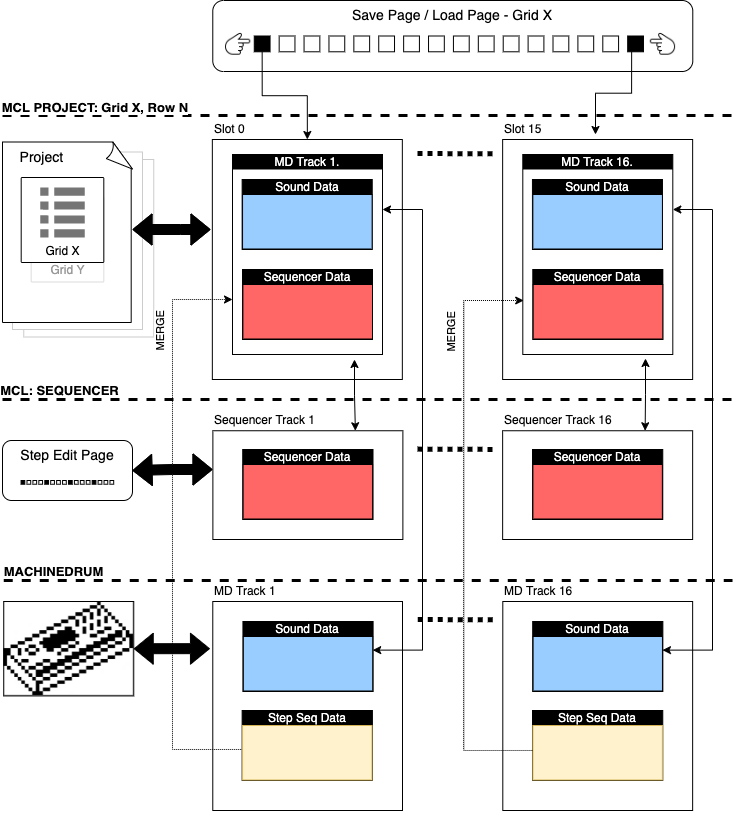
\includegraphics[scale=0.6]{save_or_load_grid_x.png}
    \caption{Save Page / Load Page - Grid X - MD }
    \label{fig:my_label}
\end{figure}
\newpage
\begin{figure}
    \centering
    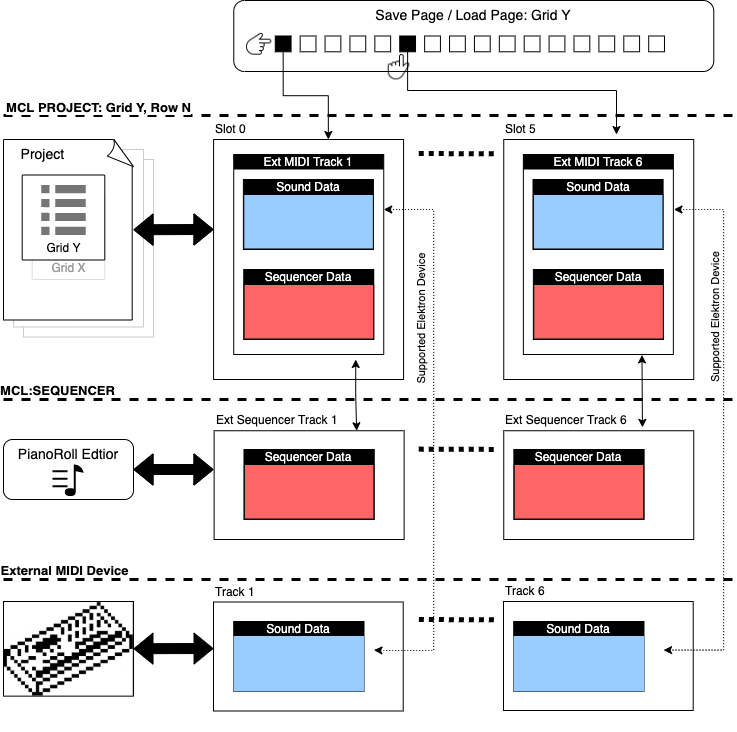
\includegraphics[scale=0.6]{save_or_load_grid_y.png}
    \caption{Save Page / Load Page - Grid Y - External MIDI}
    \label{fig:my_label}
\end{figure}
\newpage
\begin{figure}
    \centering
    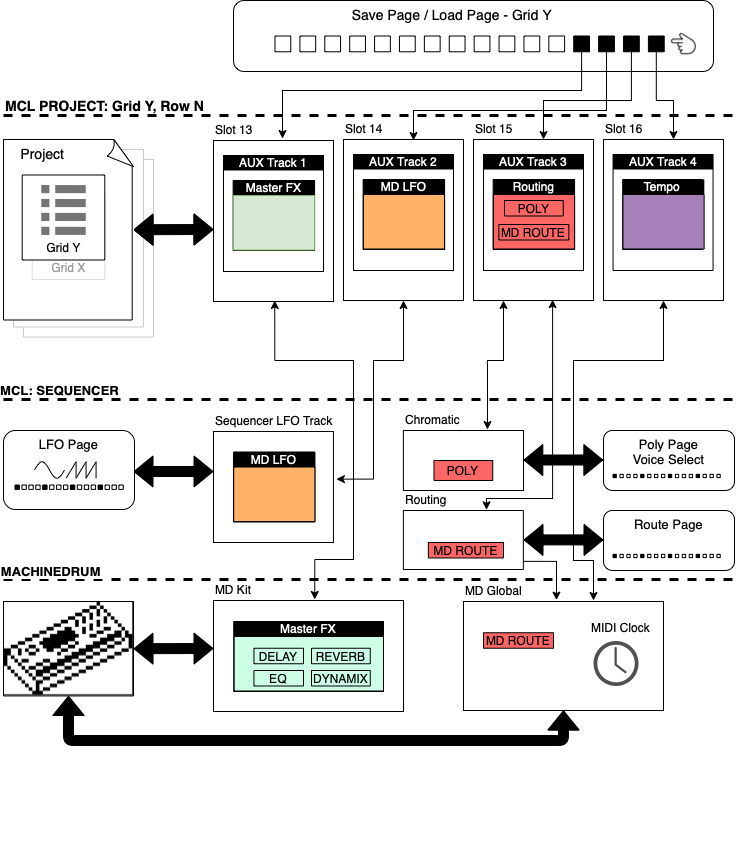
\includegraphics[scale=0.6]{save_or_load_grid_y_md.png}
    \caption{Save Page / Load Page - Grid Y - Auxiliary}
    \label{fig:my_label}
\end{figure}
